\documentclass[11pt,reqno]{amsart}
\usepackage[T1]{fontenc}
\usepackage{lmodern}
\usepackage{amsmath,amssymb,mathtools}
\usepackage[margin=1.08in]{geometry}
\usepackage{tikz}
\usepackage[hidelinks]{hyperref}
\raggedbottom

\newtheorem{theorem}{Theorem}
\newtheorem{lemma}[theorem]{Lemma}
\newtheorem{proposition}[theorem]{Proposition}

\title[Multiplicity two in planar network flow]{Multiplicity two in a tangent flow of an embedded planar network}
\author{Kaiwen Jin}
\email{yui.ui.siki@gmail.com}
\subjclass[2020]{53E10, 35K55}
\keywords{curvature flow, planar network, tangent flow, multiplicity}
\hypersetup{pdfauthor={Kaiwen Jin},pdftitle={Multiplicity two in a tangent flow of an embedded planar network}}

\begin{document}

\begin{abstract}
We construct a smooth embedded network in a disk whose first singularity
under curvature flow has a shrinking tangent flow with multiplicity two.
The network has six triple junctions and four fixed boundary endpoints.
The shrinking tangent has the two arcs of a symmetric lens and its
diameter, each with weight one. Its two exterior rays have weight two.
This gives a counterexample to the multiplicity-one conjecture for
planar network flow. A local minimum of Gaussian length in a symmetric
fixed-area class keeps the normalized evolution near the lens profile,
and a comparison for the area between the outgoing branches excludes
premature collapse of the short connectors.
\end{abstract}

\maketitle

\section{Introduction}
In planar network flow the normal velocity of each arc is its curvature,
and arcs meet at \(120^\circ\) triple junctions. Several arcs of an embedded
network can approach the same image in a blow-up at a singular point.
Arclength varifolds record the number of such arcs.

The multiplicity-one conjecture asks whether every shrinking tangent
flow of a regular embedded planar network is embedded and has weight
one \cite[Open Problem~10.1]{survey}. For the fixed-endpoint
flow in a bounded strictly convex domain, the conjecture holds when
the initial network has at most two triple junctions. It also holds
for trees whose junctions stay uniformly separated from one another
and from the fixed vertices \cite[Theorem~2.11]{mnp}. Reflection symmetry
across two perpendicular axes also allows a detailed description of
singular times in the two-junction case \cite{sym}. One familiar
shrinking limit is the symmetric lens, bounded by two curved arcs
and with a horizontal ray at each end \cite{lens}. We use its
profile to construct a flow with two bounded cells.

For an embedded network \(\Gamma\), \(V_\Gamma\) integrates
arclength along its arcs with the unoriented tangent line attached to each
point. We test against continuous compactly supported functions of
position and tangent line. A dilation includes the corresponding change
of arclength.

\begin{theorem}\label{thm:main}
There exists a smooth embedded network with six triple junctions in a
disk whose curvature flow, with \(120^\circ\) junctions and four fixed
boundary endpoints, first becomes singular at \(T=1/2\). The origin
is an interior singular point. For every sequence
\(\lambda_j\to\infty\) and every fixed \(s<0\),
\[
 V_{\lambda_j\Gamma(T+s/\lambda_j^2)}
 \ \longrightarrow\ \sqrt{-2s}\,\mathcal L
\]
locally as varifolds. The varifold \(\mathcal L\) is the sum of the
two bounded arcs of the ordinary symmetric lens at time \(-1/2\),
its horizontal diameter, and its two exterior rays. The bounded
arcs and diameter have weight one. Each exterior ray has weight two.
\end{theorem}

\begin{figure}[ht]
\centering
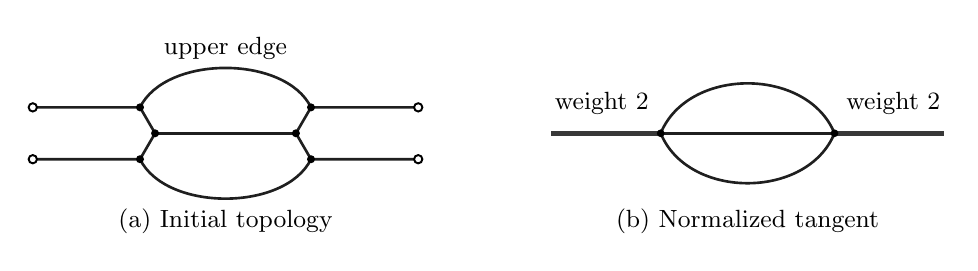
\begin{tikzpicture}[x=.89cm,y=.89cm,edge/.style={line width=.95pt,draw=black!88},
 rayheavy/.style={line width=2pt,draw=black!78}]
 \begin{scope}[shift={(-3.75,0)}]
  \draw[edge] (-2.75,.37)--(-1.22,.37)
    ..controls (-.85,1.12) and (.85,1.12)..(1.22,.37)--(2.75,.37);
  \draw[edge] (-2.75,-.37)--(-1.22,-.37)
    ..controls (-.85,-1.12) and (.85,-1.12)..(1.22,-.37)--(2.75,-.37);
  \draw[edge] (-1.22,.37)--(-1.005,0)--(-1.22,-.37);
  \draw[edge] (1.22,.37)--(1.005,0)--(1.22,-.37);
  \draw[edge] (-1.005,0)--(1.005,0);
  \foreach \u/\v in {-1.22/.37,1.22/.37,-1.22/-.37,1.22/-.37,-1.005/0,1.005/0}
    \fill[black] (\u,\v) circle[radius=1.45pt];
  \foreach \u/\v in {-2.75/.37,2.75/.37,-2.75/-.37,2.75/-.37}
    \draw[fill=white,line width=.7pt] (\u,\v) circle[radius=1.5pt];
  \node[above] at (0,.92) {\small upper edge};
  \node at (0,-1.25) {\small (a) Initial topology};
 \end{scope}
 \begin{scope}[shift={(3.7,0)}]
  \draw[rayheavy] (-2.8,0)--(-1.24,0) (1.24,0)--(2.8,0);
  \draw[edge] (-1.24,0)--(1.24,0);
  \draw[edge] (-1.24,0)..controls (-.85,.95) and (.85,.95)..(1.24,0)
                        ..controls (.85,-.95) and (-.85,-.95)..(-1.24,0);
  \fill[black] (-1.24,0) circle[radius=1.4pt];
  \fill[black] (1.24,0) circle[radius=1.4pt];
  \node[above] at (-2.08,.13) {\small weight \(2\)};
  \node[above] at (2.08,.13) {\small weight \(2\)};
  \node at (0,-1.25) {\small (b) Normalized tangent};
 \end{scope}
\end{tikzpicture}
\caption{The six-junction initial topology and its weighted limit.
Open circles mark the fixed endpoints in (a). Each triple of vertices
on one side coalesces in the normalized tangent in (b). The two rays
shown in heavier lines have weight two.}
\label{fig:network}
\end{figure}

The initial topology is shown in Figure~\ref{fig:network}. The two
bounded cells share the horizontal segment. At either end of that
segment, two short connectors join its vertex to the upper and lower
vertices. The limit is degenerate because these connectors have
vanishing length even in the normalized coordinates. The theta
nonexistence theorem of Baldi, Haus and Mantegazza \cite{theta}
concerns regular two-junction shrinkers. Chang \cite[Theorem~1.3]{chang}
changes the tangent of a regular shrinker with two or more bounded
regions by perturbing the relative cell areas. Reflection symmetry keeps
our two cell areas equal throughout the flow.
Pluda and Pozzetta \cite[Theorem~1.1]{pp} treat uniqueness for compact
nondegenerate blow-ups of networks without endpoints. Here the limiting
connectors collapse and the four exterior branches become unbounded
under rescaling. Bellettini and Novaga \cite[\S6.2]{bn} give a
premature collision for a double bubble with moving contact points
and different contact angles.

The cell area law fixes a candidate extinction time. To reach it with
the prescribed topology, we use Gaussian length in coordinates scaled
by the remaining time. Fixing the rescaled cell area removes the
dilation variation of the lens. The remaining variations increase
Gaussian length locally, including variations of the height of the
short connectors. This confines the evolving network to a neighborhood
of the lens. An earlier singularity would require the connectors on a
side to disappear while the two cells still have positive areas.
At a collapse site with a repeated-ray tangent, estimates for the tangent
angle localize all three vertices to a region smaller than the
parabolic scale. A scalar comparison for the area between the outgoing
arcs then precludes their coincidence at that scale.

\section{The symmetric network and its Gaussian length}
\label{sec:flow}

Let \(U\) denote the upper graph of the ordinary symmetric lens at time
\(-1/2\), centered at the origin. Schn\"urer et al.~\cite[Theorem~1.2 and
Proposition~5.1]{lens} give its existence and uniqueness in the class of
symmetric convex lens shrinkers. Thus \(U\) is even on \([-b,b]\), positive
in the interior, and
\begin{equation}
 U(b)=0,\qquad U'(b)=-\sqrt3,\qquad
 \frac{U''}{1+U'^2}=xU'-U .
 \label{eq:lens}
\end{equation}
The radial exterior rays of the ordinary lens begin at \((\pm b,0)\).

\begin{lemma}\label{lem:radius}
Write \(m=U(0)\). Then \(\int_0^b U\,dx=\pi/6\),
\(m\le b/\sqrt3\), and \(1<b\le\sqrt2\).
\end{lemma}

\begin{proof}
Integrating \((\arctan U')'=xU'-U\) from \(0\) to \(b\) gives the
integral formula. On the right half of the upper arc the radius increases.
Indeed the midpoint is the radial minimum in the symmetric lens construction,
and adjacent radial extrema subtend at least \(\pi/2\) at the origin
\cite[proof of Proposition~5.5]{lens}. No radial maximum can lie in the open quadrant
between that minimum and \((b,0)\).

Let \(\vartheta\in[0,\pi/3]\) be the clockwise inclination of the tangent
along this half-arc and \(w>0\) its curvature magnitude. The shrinker
equation gives \(w e^{-|X|^2/2}=\mathrm{const}\), so \(w\) is increasing.
Since \(d\vartheta=w\,d\ell\) for arclength \(\ell\),
\[
 b=\int_0^{\pi/3}\frac{\cos\vartheta}{w(\vartheta)}\,d\vartheta,
 \qquad
 m=\int_0^{\pi/3}\frac{\sin\vartheta}{w(\vartheta)}\,d\vartheta .
\]
The functions \(1/w\) and \(\cot\vartheta\) are both decreasing. Their
nonnegative covariance in the measure \(\sin\vartheta\,d\vartheta\)
bounds \(b/m\), the average of \(\cot\vartheta\) with weight
\(\sin\vartheta/w\), from below by its average with weight
\(\sin\vartheta\), which is \(\sqrt3\). Also, \(xU'-U\) decreases from \(-m\)
and \(U''\le-m\) on the right half, by \eqref{eq:lens}. Consequently
\(U(x)\le m(1-x^2/2)\), which at \(b\) implies \(b\le\sqrt2\).
Integration now gives
\[
 \frac{\pi}{3}\le 2bm(1-b^2/6)
 \le \frac{2b^2}{\sqrt3}(1-b^2/6).
\]
For \(b\le1\), the last expression is at most \(5/(3\sqrt3)<\pi/3\).
\end{proof}

\subsection{Compatible initial data and the area law}

We impose reflection symmetry across both axes. The three right-hand
vertices are \((c,0)\) and \((a,\pm h)\) with \(a,c,h>0\). The two
connectors join \((c,0)\) to \((a,\pm h)\). The upper and lower
curved edges join the reflected upper and lower vertices, respectively.
The central edge joins \((-c,0)\) to \((c,0)\). Each of the four
vertices off the horizontal axis has an exterior edge. Fix \(L>b+1\)
large enough to contain the bounded lens with a margin. For a small
\(h_{\rm end}>0\) put the fixed endpoints at \((\pm L,\pm h_{\rm end})\)
on the disk of radius \((L^2+h_{\rm end}^2)^{1/2}\).

Initially choose \(h=h_{\rm end}\), \(c=b\), \(a=b+h/\sqrt3\), and use
straight connectors and horizontal exterior edges. In the upper right
quadrant set \(x=q(y)\), \(0\le y\le h\), on the connector. Start the
upper edge there with the graph \(h+U(\zeta(x))\), \(0\le x\le a\),
where
\[
 \zeta(x)=x-(a-b)\chi(x)
\]
and \(\chi\) is a smooth nondecreasing cutoff equal to zero near \(0\)
and one near \(b\). Then \(\zeta(a)=b\) and \(0<\zeta'\le1\) for small
\(h\). Interpolate the graph's derivative to \(-\sqrt3\) in a shrinking
neighborhood of \(a\) and integrate back from its endpoint height
\(h\). The resulting graph \(u\) has \(-\sqrt3\le u_x\le0\) and a
straight germ at \(a\). Add a smooth bump supported strictly inside
\((0,b)\) to make
\begin{equation}
 \int_0^a u(x)\,dx-\int_0^h yq_y(y)\,dy=\frac{\pi}{6}.
 \label{eq:initial-area}
\end{equation}
The bump has nonzero integral and can be taken with coefficient tending
to zero as \(h\downarrow0\), since the expression on the left tends
to \(\int_0^b U\). The support can be chosen where \(U'\) lies strictly
between \(-\sqrt3\) and \(0\), so the slope bound persists. Reflection
completes the graph. Its upper central arc has height \(>h\) in the
open \(x\)-interval, the upper exterior edges lie at height \(h\),
and the upper connectors lie between heights \(0\) and \(h\).
The resulting network is embedded with \(120^\circ\) angles. Choose
parameters affine on each straight germ. The higher spatial derivatives
vanish there, so \(\gamma_t=\gamma_{xx}/|\gamma_x|^2\) gives vanishing
time derivatives of all positive orders at the fixed endpoints and
junctions. This gives the compatibility conditions.

Let \([0,S)\) be the maximal regular smooth existence interval.
Existence and geometric uniqueness for these data follow from
\cite[Theorem~3.29 and Corollary~3.34]{survey}. In particular the
reflections persist, and the flow stays embedded in the disk
\cite[Proposition~8.12]{survey}. The central edge is fixed as a set by
horizontal reflection and its endpoints are individually fixed by that
reflection. The induced involution on the edge is increasing and hence
is the identity. The edge therefore lies on the horizontal axis.

The left side of \eqref{eq:initial-area} is the area of the right half
of the upper cell by Green's formula. Each full cell has four convex
\(120^\circ\) corners. For a positively oriented cell boundary, area
differentiation gives minus the integral of signed curvature, and
the four corners contribute \(4\pi/3\) to the total turn \(2\pi\).
Both cell areas are therefore
\begin{equation}
 A(t)=\frac{\pi}{3}-\frac{2\pi}{3}t
      =\frac{2\pi}{3}(T-t),\qquad T=\frac12 .
 \label{eq:area-law}
\end{equation}
Since the cells have positive area on the regular interval, \(S\le T\).

\subsection{Graph bounds}

Follow the upper edge from its vertical-axis midpoint to \((a,h)\) and
orient the upper connector from the axis to \((a,h)\). Orient the right
exterior edge outward. If \(\alpha\) is the real tangent angle in each
orientation, use the angle variable \(\Theta=\alpha+\pi/3\) on the upper
edge, \(\Theta=\alpha-\pi/3\) on the connector, and \(\Theta=\alpha\)
on the exterior edge. The \(120^\circ\) condition makes these agree
at their common junction. With arclength \(\ell\) and tangential
speed \(\lambda\), \(\Theta_t=\Theta_{\ell\ell}+\lambda\Theta_\ell\)
on each edge \cite[\S3 and (8.4)]{ins}. The sum of the outgoing
derivatives of \(\Theta\) at the junction is zero, since the outgoing
curvatures are the normal projections of the same vertex velocity.
The boundary values are \(\Theta=\pi/3\) at the midpoint by reflection
and \(\Theta=0\) on the connector at the axis. At the fixed endpoint
\(\Theta_\ell=0\) because \(k=0\). To prove the upper bound, test \(\Theta-\varepsilon(1+t)\) at a first
contact with \(\pi/3\). At a junction maximum all outgoing derivatives
are nonpositive and sum to zero. Thus each is zero and each one-sided
second derivative is nonpositive, contradicting the strict differential
inequality. The open-edge and Neumann endpoint tests give the same
contradiction. Apply the test to \(-\Theta-\varepsilon(1+t)\) at level
zero for the lower bound and let \(\varepsilon\downarrow0\).

Thus the upper arc and the exterior edge are graphs \(y=u(x,t)\)
and \(y=f(x,t)\) on \([0,a]\) and \([a,L]\). The connector is a graph
\(x=q(y,t)\) on \([0,h]\). They satisfy
\begin{equation}
 -\sqrt3\le u_x\le0,\qquad 0\le f_x\le\sqrt3,\qquad
 |q_y|\le1/\sqrt3,\qquad q_y(0,t)=1/\sqrt3 .
 \label{eq:slopes}
\end{equation}
These conclusions hold as long as the vertices and symmetry
sections remain in their indicated quadrants. The bounds established
below keep \(a,c\) positive, and embeddedness prevents the two
reflected vertices \((a,\pm h)\) from coinciding on the regular
interval. The physical central vertex coordinate \(c(t)=q(0,t)\)
is nonincreasing. Indeed,
\begin{equation}
 c'(t)=\frac{q_{yy}(0,t)}{1+q_y(0,t)^2}\le0,
 \label{eq:c}
\end{equation}
using the graph equation and the one-sided maximum of \(q_y\) at \(0\).
We also have \(|a-c|\le h/\sqrt3\). At all times on the chart, the
right half of the upper cell has the same area formula as in
\eqref{eq:initial-area}, by Green's formula even if \(q\) is not
monotone.

\subsection{Gaussian monotonicity with fixed endpoints}

Normalize about the origin by \(X=x/\sqrt{2(T-t)}\) and
\(\sigma=-\frac12\log(2(T-t))\), using the prescribed \(T\) from
\eqref{eq:area-law}. In normalized coordinates the curvature is
\(\widetilde k\) and \(X_\sigma\cdot\nu=\widetilde k+X\cdot\nu\).
For \(g(X)=e^{-|X|^2/2}\), differentiation of \(g\,d\ell\) and
integration by parts give the Gaussian integral term
\(-\int g|\widetilde k+X\cdot\nu|^2\,d\ell\) and boundary term
\(g V\cdot T_{\rm out}\), with \(V=X_\sigma\) and \(T_{\rm out}\)
directed toward the endpoint of the arclength interval. The three
terms cancel at each triple vertex. At a fixed physical endpoint
its normalized position \(P\) satisfies \(P_\sigma=P\), so its
boundary term is \(g(P)P\cdot T_{\rm out}\).

Add to the Gaussian length the four radial integrals
\(\int_{|P|}^\infty e^{-r^2/2}\,dr\), one from each normalized fixed
endpoint. Each has derivative \(-g(P)|P|\). Thus the sum of the
boundary terms and radial derivatives is nonpositive. Denote a quarter
of this augmented Gaussian length by \(\mathcal F\). We have
\begin{equation}
 \frac{d}{d\sigma}\mathcal F\le0.
 \label{eq:monotone}
\end{equation}
The radial integrals are used only in this functional.
By \eqref{eq:area-law} the normalized upper-right half-cell area is
exactly \(\pi/6\).

\section{A local minimum of Gaussian length}\label{sec:coercivity}

In this section \(a,c,h,u,f,q\) denote normalized graph
coordinates, and the right endpoint of \(f\) is \((l,f(l))\).
Write \(G(x)=e^{-x^2/2}\). Let \(\mathcal F_*\) be a quarter
of the Gaussian length of the normalized limit described in
Theorem~\ref{thm:main}. The axis in the upper-right contribution
carries half the weight of an off-axis edge. Because the appended
exterior path starts at radius \(\sqrt{a^2+h^2}\) and goes to infinity,
its Gaussian length is at least
\(\int_{\sqrt{a^2+h^2}}^\infty G(r)\,dr\), by \(ds\ge dr\).

\begin{proposition}\label{prop:coercive}
There are \(\delta_0,\gamma>0\) with the following property. Suppose the
symmetric graphs satisfy \eqref{eq:slopes}, have upper-right cell area
\(\pi/6\), and \(|a-b|+h+\|\phi-U\|_\infty<\delta_0\), where
\(\phi(x)=u(ax/b)\) on \([0,b]\). Then
\begin{equation}
 \mathcal F-\mathcal F_*
 \ge \gamma\left((a-b)^2+h^2+\|\phi-U\|_{H^1(0,b)}^2\right).
 \label{eq:coercive}
\end{equation}
\end{proposition}

\begin{proof}
Since \(q(0)=c\) and \(q(h)=a\), we may replace the half-axis integral
\(\tfrac12\int_0^c G\) by
\(\tfrac12\int_0^a G-\tfrac12\int_0^h G(q)q_y\,dy\).
The sum of the connector and half-axis contributions is
\[
 \frac12\int_0^a G(x)\,dx+
 \int_0^h G(q(y))\left(e^{-y^2/2}\sqrt{1+q_y^2}-q_y/2\right)\,dy .
\]
The function \(p\mapsto\sqrt{1+p^2}-p/2\) is strongly convex on the
allowed slope interval and has minimum \(\sqrt3/2\) at \(p_*=1/\sqrt3\).
Since \(|q(y)-a|\le h/\sqrt3\),
\[
 \frac{G(q(y))}{G(a)}=1+a(a-q(y))+O(h^2),\qquad
 \int_0^h (a-q(y))\,dy=\int_0^h y q_y(y)\,dy.
\]
Replacing \(q_y\) by \(p_*\) in this last integral makes an error bounded
by \(Ch^{3/2}\|q_y-p_*\|_2\). The convexity surplus absorbs this by
Young's inequality at cost \(Ch^3\). The factor \(e^{-y^2/2}\) changes
the integral by at most \(Ch^3\). Therefore \(\mathcal F\ge E-Ch^3\),
where
\begin{align}
 E(a,h,u)={}&
 \int_0^a e^{-(x^2+u^2)/2}\sqrt{1+u_x^2}\,dx
 +\frac12\int_0^a G(x)\,dx
 +\int_{\sqrt{a^2+h^2}}^\infty G(r)\,dr \notag\\
 &+G(a)\left(\frac{\sqrt3}{2}h+\frac a4h^2\right).
 \label{eq:effective}
\end{align}
Here \(E(b,0,U)=\mathcal F_*\).

To differentiate at the ordinary lens, transport the upper arc to
the fixed interval by \(\phi(x)=u(ax/b)\). Along a smooth variation
let \(A=\dot a,\ H=\dot h\), and \(v=\dot\phi-(A/b)xU'\). The latter
is the first variation at fixed horizontal position. The endpoint and
area constraints give
\begin{equation}
 v(b)=H+\sqrt3 A,\qquad \int_0^b v\,dx=0.
 \label{eq:variation-constraint}
\end{equation}
The first identity comes from \(u(a)=h\). For the second, differentiate
\((a/b)\int_0^b\phi\), using \(U(b)=0\) and the \(O(h^2)\) connector
area. After integration by parts in the upper graph, the first variation
of \(E\) is the sum of its four endpoint contributions,
\[
 G(b)\left(\frac{A-\sqrt3 H}{2}+\frac A2-A+\frac{\sqrt3 H}{2}\right)=0 .
\]
This cancellation uses only the endpoint condition. Set \(\rho=e^{-(x^2+U^2)/2}\), \(W=\rho/\sqrt{1+U'^2}\) and
\(M=\rho/(1+U'^2)^{3/2}\). The second variation is
\begin{equation}
 Q(v,H)=
 \int_0^b(Mv'^2-Wv^2)\,dx-\frac b2G(b)v(b)^2
 +G(b)(b-b^{-1})H^2 .
 \label{eq:hessian}
\end{equation}
For the boundary terms, put
\(L(x,u,p)=e^{-(x^2+u^2)/2}\sqrt{1+p^2}\).
Its Euler equation at \(U\) gives \(L_{uu}-(L_{up})'=-W\),
\(L_{pp}=M\), and \(L_{up}=0\) at both ends. At \(b\) the
values of \(L,L_p,L_x\) are \(2G(b),-\sqrt3 G(b)/2,-2bG(b)\).
Differentiating \(u(a)=h\) twice at the lens gives
\[
 \ddot u(b)+2Av'(b)+A^2U''(b)+\ddot a\,U'(b)=\ddot h ,
\]
with \(\ddot u\) evaluated at fixed position. The \(L_p(b)\ddot u(b)\)
term from integration by parts cancels \(2A L_p(b)v'(b)\) from the
moving upper limit. The upper graph then contributes the integral in
\eqref{eq:hessian}, together with
\[
 G(b)\left(-2bA^2+\tfrac12(\ddot a-\sqrt3\,\ddot h)\right).
\]
The axis, radial integral and connector terms in \eqref{eq:effective}
contribute respectively, after dividing by \(G(b)\),
\[
 \tfrac12(\ddot a-bA^2),\qquad
 -\ddot a-H^2/b+bA^2,\qquad
 \tfrac{\sqrt3}{2}\ddot h-\sqrt3 bAH+bH^2/2 .
\]
They cancel the accelerations. Inserting
\(v(b)=H+\sqrt3 A\) gives the last two terms of \eqref{eq:hessian}.

We check positivity of the first two terms of \eqref{eq:hessian}
on the area constraint. The function \(D=U-xU'>0\) satisfies
\((MD')'/W+D=2D\), with \(D'(0)=0\) and \(D'(b)=4bD(b)\).
These identities follow by differentiating \eqref{eq:lens}, or by
differentiating \(\mu U(x/\mu)\) under the normalized graph equation
with \(\mu_\sigma=\mu-\mu^{-1}\) at \(\mu=1\).
The curvature first integral gives \(WD=\mathrm{const}\).
Hence \(\int v=0\) is weighted orthogonality to \(D\) in
\(L^2(W\,dx)\). On writing \(v=D z\), integration by parts gives
\[
 \int_0^b(Mv'^2-Wv^2)\,dx-\frac b2G(b)v(b)^2
 =\int_0^b MD^2 z'^2\,dx-2\int_0^b WD^2 z^2\,dx .
\]
With arclength \(\ell\) along the quarter lens, \(WD^2\,dx\) is
a positive constant times \(e^\psi d\ell\), where \(\psi=|X|^2/2\).
Since \(M/W=(1+U'^2)^{-1}\), the derivative term becomes
\(MD^2 z'^2\,dx=WD^2|z_\ell|^2\,dx\), with the same measure.
The mean of \(z\) in this measure is zero.
Let \(B\) be the quarter-lens length. The first positive Neumann
eigenvalue of \(-\partial_{\ell\ell}-\psi_\ell\partial_\ell\) on
\([0,B]\) is at least \(\pi^2/B^2-1/2\). To see this, differentiate
the equation for its first nonconstant eigenfunction and multiply
the derivative by \(e^{\psi/2}\). This gives a Dirichlet eigenfunction
with potential \(\psi_\ell^2/4-\psi_{\ell\ell}/2\ge-1/2\), since
\(\psi_{\ell\ell}=1-k^2\). Apply the Dirichlet interval inequality.
The first nonconstant weighted eigenfunction exists by minimizing the
Rayleigh quotient under the weighted mean-zero and unit-norm
constraints. Now \(\sqrt{1+p^2}\le1+|p|/\sqrt3\) on
\(|p|\le\sqrt3\), so Lemma~\ref{lem:radius} gives
\(B\le b+m/\sqrt3\le4\sqrt2/3\). The spectral lower bound is
\(9\pi^2/32-1/2>2\). Thus \(Q(v,H)>0\) for each nonzero variation
satisfying \eqref{eq:variation-constraint}, using \(b>1\).

Finally we justify the use of the quadratic form with only uniform
closeness and bounded slopes. On \([0,b]\) the arc integrand is
\[
 \frac{a}{b}\exp\!\left(-\frac{(ax/b)^2+\phi^2}{2}\right)
       \sqrt{1+(b\phi'/a)^2}.
\]
It is smooth in \((a,\phi,\phi')\) and uniformly convex in \(\phi'\)
on the given bounded slope range. Taylor expand the terms independent
of the slope increment and the coefficient linear in that increment.
Uniform convexity bounds the remaining term below. The zero first
variation and Young's inequality give
\[
 E-E_*\ \ge\ c\|(\phi-U)'\|_2^2
          -C\big((a-b)^2+h^2+\|\phi-U\|_2^2\big).
\]
If \eqref{eq:coercive} failed, take a sequence with uniform distance
going to zero and with \((\mathcal F-\mathcal F_*)/r_j^2\) of
nonpositive limsup, where \(r_j^2=(a-b)^2+h^2+\|\phi-U\|_{H^1}^2\).
The preceding bound and \(\mathcal F\ge E-Ch^3\) imply that \(r_j^2\)
is bounded by a constant times \((a-b)^2+h^2+\|\phi-U\|_2^2\).
In particular \(r_j\to0\). After division by \(r_j\), the endpoint
and fixed-interval graph increments converge along a subsequence
to \((A,H,\xi)\ne0\), with \(\xi\) the uniform and weak \(H^1\) limit
of the graph increment. The corresponding variation at fixed horizontal
position is \(v=\xi-(A/b)xU'\). Taking the first-order parts of the endpoint
and area identities gives \eqref{eq:variation-constraint} for \((v,H)\).

For the slope-square term of the normalized increment, use the Taylor
coefficient at the reference graph on \(|(\phi-U)'|\le\varepsilon\)
up to its uniform modulus of continuity. On the complement keep the
nonnegative convexity remainder. This complement has measure
\(O(r_j^2/\varepsilon^2)\), so the normalized derivative on it converges
weakly to zero in \(L^2\). Weak lower semicontinuity and then
\(\varepsilon\downarrow0\) give the slope-square contribution of
\eqref{eq:hessian}. The mixed terms converge by uniform convergence
of the normalized undifferentiated differences and weak convergence
of the normalized derivatives. Hence the liminf of
\((E-E_*)/r_j^2\) is at least \(Q(v,H)/2>0\). The error \(Ch^3/r_j^2\)
tends to zero. This contradicts the selected sequence.
\end{proof}


\section{The first singular time}\label{sec:lifetime}

Choose a small \(\delta<\delta_0\) from Proposition~\ref{prop:coercive}
with \(b-\delta>1\) and \(a-h/\sqrt3>0\) for
\(|a-b|+h\le\delta\). The initial normalized scale is one. By the choice
of initial \(h_{\rm end}\) we can make both
\[
 d=|a-b|+h+\|u(a\,\cdot/b)-U\|_\infty,\qquad
 \mathcal F-\mathcal F_*
\]
arbitrarily small at \(t=0\). For \(d\le\delta\),
\eqref{eq:coercive} and the one-dimensional Sobolev inequality give
\(\mathcal F-\mathcal F_*\ge C_0 d^2\) with \(C_0>0\) fixed.
Choose data with \(d(0)<\delta/2\) and
\(\mathcal F(0)-\mathcal F_*<C_0\delta^2/4\).
Then a first exit \(d=\delta\) contradicts \eqref{eq:monotone}.
The chart used for this test persists up to such an exit by
\eqref{eq:slopes}, the bounds on \(a,c\), and embeddedness.
We fix this choice of data, taking \(\delta\) small enough also for
the estimate in Section~\ref{sec:tangent}.

Suppose \(S<T\). In the rest of this section \(a,c,h,u,q,f\) are
in physical coordinates. The scale \(\sqrt{2(T-t)}\) is bounded
above and below by positive constants for \(t<S\), so \(a,c\)
stay away from zero and \(a\) stays a positive distance from \(L\).
Both simple cell areas and the area of their union have positive
lower bounds. These are all the simple cycles of the graph.
Their lengths are bounded below, since a closed boundary of length
\(m\) and the region it encloses lie in a ball of radius \(m/2\)
centered at a boundary point.

We first verify that the vertices have limits at \(S\).
Set \(I=\int_\Gamma k^2\,d\ell\), \(J_1=\int_\Gamma k_\ell^2\,d\ell\)
and \(K=\|k\|_\infty\), at each time. Total length dissipation gives
\(\int_0^S I\,dt<\infty\). At a fixed time cut one point of each
remaining simple cycle where \(k^2\) is at most its average on the
cycle. This gives a finite forest whose new leaf values obey
\(k^2\le CI\). Original endpoints have \(k=0\). Root the tree containing
a maximum point of \(k^2\) at that point. Integrate
\((k^2)_\ell=2k k_\ell\) toward its leaves, bounding the incoming
square at each junction by twice the sum of the two outgoing squares.
The leaf bounds and Cauchy--Schwarz give \(K^2\le C(\sqrt{I J_1}+I)\).
These tree estimates use the junction calculation of \cite[\S4]{mnp}.
The curvature energy inequality is
\begin{equation}
 I'\le -2J_1+K^2 I+CK^3 .
 \label{eq:energy-early}
\end{equation}
To obtain it, use \(k_t=k_{\ell\ell}+\lambda k_\ell+k^3\) and
\((d\ell)_t=(\lambda_\ell-k^2)d\ell\). The boundary term on an
oriented interval is \([2k k_\ell+\lambda k^2]\).
The common time derivative of the angle at a triple point is
\(k_\ell+\lambda k\) in the outgoing coordinates on each arm.
The three \(k\)'s sum to zero, so only a cubic boundary contribution
bounded by \(CK^3\) remains. At the fixed endpoints the term vanishes.
Young's inequality with \(Z=1+I\) gives
\(Z'\le -J_1+CZ^3\), hence \(J_1/Z^2\le (1/Z)'+CZ\).
Both \(\int_0^S Z\,dt\) and \(\int_0^S J_1/Z^2\,dt\) are finite.
The interpolation bound now gives
\(K\le C[Z^{1/2}+Z^{3/4}(J_1/Z^2)^{1/4}]\), which is integrable.
Since a triple velocity is determined by its three normal projections
and the normals are at \(120^\circ\), each vertex velocity is bounded
by \(CK\). This gives the vertex limits.

\subsection{Good slices and the case of positive limiting height}
\label{sec:goodslices}

We use parabolic compactness \cite[Definition~8.4 and
Proposition~8.17]{survey} in the following form. At a point \(x_0\)
and terminal time \(S\), take a subsequence of spatial dilations
\(\lambda_j\to\infty\) with a single possibly degenerate shrinking
limit flow. At almost every \(s<0\), the curves of
\[
 \Gamma_j(s)=\lambda_j\bigl(\Gamma(S+s/\lambda_j^2)-x_0\bigr)
\]
converge locally in \(C^{1,\alpha}\cap W^{2,2}\), \(0<\alpha<1/2\).
The curve convergence is on indexed branches and retains their arclength
even where their images meet. Choose the good slices from this full-measure
set where also the Gaussian defect
\(\int |k\nu-X^\perp/(2s)|^2\rho_{0,0}\,d\ell\) tends to zero, as in the
proof of the proposition, with
\(\rho_{0,0}(X,s)=(4\pi|s|)^{-1/2}e^{-|X|^2/(4|s|)}\).
Square curvature integrals are then uniformly
bounded on compact sets. Formula (8.9) of \cite{survey} computes terminal
Gaussian density with the arclength of every limiting branch. Each
radial ray from the center contributes \(1/2\) per label. The interior
density threshold for local regularity is \(3/2\)
\cite[Corollary~9.5]{survey}.
The boundary version uses the threshold \(3/4\) and reflection at the
fixed endpoint \cite[Corollary~9.6]{survey}.

A nonzero-curvature shrinker edge lies in a bounded set. For example,
at time \(-1/2\) we have \(k\nu=-X^\perp\),
\(k_\ell=(X\cdot T_{\rm tan})k\), and
\(|k|\le |X|\), so a nonzero constant value of \(k e^{-|X|^2/2}\)
bounds \(|X|\). At other negative times one rescales this identity.
Thus an edge unbounded in its graph coordinate is straight and
radial. A graphical branch with projected endpoints tending to both
infinities gives at most one line.

Suppose \(h(S)>0\). The six terminal vertices are distinct.
Away from them and the fixed endpoints there is at most one
graphical sheet locally at late times. Indeed, the upper and exterior
\(x\)-graphs both have height at least \(h(t)\) and partition the
horizontal interval at \(a(t)\). A connector has height between
\(0\) and \(h(t)\) and reaches either extreme only at its endpoint.
The two connectors in the upper half-plane are separated horizontally:
each is within \(h(t)/\sqrt3\) of the horizontal coordinate of its top
vertex, and the normalized trapping radius can be taken smaller than
this separation margin. The lower half-plane is obtained by reflection.
Any nonempty tangent away from the vertex and endpoint limits is
therefore a single line.

At the upper right terminal vertex, near its limit there are only
the two \(x\)-graphs and one connector, an \(x\)-Lipschitz graph over
\(y\) ending at height \(h(t)\). Consider the horizontal and vertical
coordinates of the rescaled vertex relative to this terminal point.
If both coordinates are bounded on the good slice, the three arms remain in the limit,
are unbounded in their respective graph coordinates, and balance.
Three radial straight edges cannot balance at a point other than
the origin, where they form a triod. If scaled height tends to
\(+\infty\), the two \(x\)-graphs leave every compact set and at most
one sheet of the connector remains. If scaled height tends to
\(-\infty\), the connector is absent. Of the other two branches,
neither remains if the scaled horizontal coordinate is bounded,
by the uniform slope bound, and at most one remains if that
coordinate escapes. If height stays bounded but horizontal position
escapes, the connector escapes by its Lipschitz bound in \(y\), and
at most one of the remaining two branches is visible.
At the central terminal vertex, the connectors over the two opposite
\(y\)-halves and the axis give a triod if the scaled vertex remains
bounded. If it escapes, the two connectors leave the ball and at most
the axis remains. Reflections cover the other vertices. Thus every
interior density is at most \(3/2\).

The trapping bounds and the choice of \(L\) keep the bounded arcs
and connectors a positive distance from the disk boundary. By
\eqref{eq:slopes} and the fixed endpoint heights, the exterior graphs
lie in the rectangle with corners \((\pm L,\pm h_{\rm end})\).
Only these corners touch the disk boundary, and only one graph
approaches each corner. The fixed-point reflection of \cite[\S8.2]{survey} extends it to a
single graph across the endpoint, with tangent density one in the
reflected flow. The original boundary density is \(1/2\).
By the two density criteria, curvature is bounded on a neighborhood
of each point of the compact set of subsequential terminal support
limits, hence uniformly on the whole network near \(S\). Every edge
has a positive length lower bound from its distinct endpoints.
The continuation criterion \cite[Theorem~5.7]{survey} contradicts
maximality at \(S\).

\subsection{Vanishing connectors before extinction}\label{sec:early-collapse}

If \(h(S)=0\), the three right vertices approach \(x_0=(c_*,0)\),
where \(a(S)=c(S)=c_*>0\). The inequality \eqref{eq:c} gives
\(c(t)\ge c_*\). We need a lower bound on the incoming upper edge
even if the three vertices leave the parabolic scale to the right.
For some fixed \(\eta>0\),
\begin{equation}
 u(x,t)\ge \eta(c_*-x)\quad
 \text{for \(x<c_*\) close to \(c_*\), \(x\le a(t)\), and \(t\) near \(S\)}.
 \label{eq:incoming}
\end{equation}
On \([c_*-d_1,c_*]\) take a nonnegative profile
\(\varphi(x)=(c_*-x)\chi_1(x)\), with \(\chi_1=1\) near \(c_*\),
positive in the interior, and equal to \((x-c_*+d_1)^2\) near the
left endpoint. Choose \(0<d_1<c_*\). The function
\(\eta_0 e^{-C(t-t_0)}\varphi\) is a subsolution of the graphical
flow for large \(C\): it is affine in space near \(c_*\), its second
derivative is positive near the left edge, and \(\varphi\) has a
positive minimum on the remaining compact subinterval. Fit it below
\(u\) initially by choosing \(\eta_0>0\) small. Its value is zero at
both fixed sides. If the side \(a(t)\) lies to the left of \(c_*\),
then \(c_*-a(t)\le c(t)-a(t)\le h(t)/\sqrt3\), so the subsolution
also lies below \(u(a(t),t)=h(t)\). Comparison on the moving
intersection with \(\{x\le a(t)\}\) gives \eqref{eq:incoming}.

Write \(X=\lambda_j(x-x_0)\) and \(s=\lambda_j^2(t-S)\) for
the parabolic coordinates about \((x_0,S)\). Fix a good rescaled time
\(s_0<0\), set \(t_j=S+s_0/\lambda_j^2\), and write
\[
 c_j=\lambda_j(c(t_j)-c_*)\ge0,\qquad
 a_j=\lambda_j(a(t_j)-c_*),\qquad h_j=\lambda_j h(t_j)
\]
so \(|a_j-c_j|\le h_j/\sqrt3\).
Pass to subsequences according to whether \(h_j,c_j\) stay bounded
or escape to \(+\infty\).
\begin{itemize}
\item If \(h_j\to\infty\), all the upper and lower \(x\)-graphs are
  absent on compact sets. For \(c_j\to\infty\) the connectors escape
  by their Lipschitz bound in \(y\), leaving the axis. For bounded \(c_j\)
  the two connector branches extend to both vertical infinities and,
  with the axis, form a triod.
\item If \(h_j\) stays bounded but \(c_j\to\infty\), then \(a_j\to\infty\).
  The connectors and both exterior branches escape. If the upper
  branch is visible it yields an entire graph in the closed upper
  half-plane, since it has bounded slope and its horizontal endpoints
  leave both ends of the scaled axis. A complete radial line there
  must be the axis, contrary to \eqref{eq:incoming} at any fixed
  negative scaled \(x\). The reflected branch is absent as well,
  so only the axis remains.
\item If \(h_j,c_j\) are bounded, all three vertices and both
  connectors stay in a compact set. Each of the four \(x\)-graphs
  gives a radial straight ray. If the upper height had a positive
  limit, its two attached radial rays would be collinear at that
  nonzero point, incompatible with the third unit tangent at a
  regular triple. Hence \(h_j\to0\), the connectors have lengths
  \(O(h_j)\), and their variation of tangent tends to zero by the
  bounded scaled square curvature integral. The assigned angles at
  the axis are \(60^\circ\) and \(300^\circ\).
  A nonzero limiting position on the axis would force all four radial
  rays to be horizontal and be incompatible with those angles. At
  the origin the triple angles therefore give two coincident rightward
  rays and single rays in directions \(120^\circ,180^\circ,240^\circ\).
\end{itemize}
The line and triod alternatives give smoothness at \(x_0\), which
forbids the collapse of the three incident vertices there.
It remains to exclude the five-ray cone in the final alternative.

\paragraph{Angle propagation.}
Cut the right-hand tree at a fixed vertical line strictly to the left
of \(c_*\). The three cut endpoints and the fixed endpoints stay
a fixed positive distance from \(x_0\) in physical coordinates.
The lift \(\Theta\) on the upper half, its negative reflection below,
and zero on the axis form one real angle \(\theta\) on this tree
with \(|\theta|\le\pi/3\). At the chosen time \(s_0\), all three
rescaled vertices approach the origin. In every fixed ball the
curvature energy tends to zero because the shrinker defect tends to zero,
the noncollapsed branches converge in tangent to radial lines and
the collapsed edges have vanishing length. Paths from the middle
vertex to any point in a fixed scaled square \(Q_D=(-D,D)^2\) stay
inside a larger fixed ball. This follows from the collapsed
connectors and the fixed graph bounds on the five arms.
The corresponding angle oscillation tends to zero there by
Cauchy--Schwarz, since \(\theta_\ell=k\). Denote the initial
deviation on \(Q_D\) from the lift value at that vertex by
\(\epsilon_j(D)\).

For an ambient function \(B\), the heat operator along the evolving edge
applies to the pullback of \(B\) as
\[
 B_s-\operatorname{Hess}B(T_{\rm tan},T_{\rm tan}).
\]
For \(a_1>0\) and a constant \(M_0\) bounding the lifted deviation
globally, compare both signs to
\[
 \epsilon_j(D)+M_0 e^{a_1^2(s-s_0)}
 \sum_{i=1}^2\left(e^{a_1(X_i-D)}+e^{a_1(-X_i-D)}\right).
\]
This is a supersolution and bounds the deviation at intersections
with the fixed square boundary \(\partial Q_D\). The edge outgoing derivatives sum to zero
at each vertex for both the angle and the pullback of the barrier.
The same maximum principle as for \eqref{eq:slopes} applies.
Set \(a_1=(D-d_2)/(2|s_0|)\) to bound the deviation in \(Q_{d_2}\)
by \(\epsilon_j(D)+4M_0 e^{-(D-d_2)^2/(4|s_0|)}\).
Taking \(j\to\infty\) first and then \(D\to\infty\) makes it
uniformly small on every fixed square throughout
\([s_0,0)\).

\paragraph{Curvature near a fixed scaled cut.}
The pullback of \(|X-z|^2+2(s-s_0)\) solves the same
edge heat equation with junction flux sum zero. Its minimum on the
tree cannot fall below its initial minimum, provided the endpoint
values stay above that lower bound. The fixed physical distances of
the endpoints from \(x_0\) ensure this for each fixed scaled \(z\).
In particular, during the remaining time, no point occurs at \(z\)
if its initial distance from the network exceeds
\(\sqrt{2|s_0|}\). Initial convergence to the cone then puts
the support of the scaled flow, in any sufficiently large fixed
annulus away from its two margins, into tubes of fixed width about
the four distinct ray directions. Write \(w_0\) for their half-width.
Choose the radius large enough for the tubes to be disjoint, and
leave radial margins larger than \(10w_0\) around the smaller
annulus used for the cuts.

There are no vertices in this smaller annulus. At a vertex one
outgoing tangent has projection at least \(1/2\) on a chosen unit
normal to its tube. The uniform angle estimate maintains projection
at least \(1/4\) along that edge inside the larger annulus. At a vertex
reached along the path, continue on an outgoing arm with the same
property. The transverse height strictly increases. Within length
\(9w_0\) the path must leave its tube before reaching either margin,
contradicting support containment. The same argument in a vertex-free
collar excludes tangent lines with absolute normal projection at
least \(1/2\). At large radius the circle's tangent has normal
projection close to one in the tube, so every crossing of the
circle is transverse. All three vertices start inside it and remain
inside. The five crossings present at \(s_0\) persist on their
labels because crossings cannot meet a vertex or become tangent.

Use the corresponding ray direction as horizontal coordinate at
each cut. On a circle of radius \(\varrho\) the projected crossing
coordinates lie in \([\sqrt{\varrho^2-w_0^2},\varrho]\). Choose a
fixed \(\eta>0\) so that this interval lies within
\((\varrho-\eta,\varrho+\eta)\) and the larger interval
\((\varrho-2\eta,\varrho+2\eta)\), restricted to its tube, lies in
the vertex-free collar. This is possible by taking \(\varrho\)
large and using the radial margins. The ray projection is strictly
monotone on each strand through the collar, so each crossing belongs
to a graph over the larger fixed interval. The slopes there tend
uniformly to zero by angle propagation from \(s_0\). The interior
graphical estimates of Ecker--Huisken \cite[Theorems~3.1 and 3.4]{eh}
give bounds for \(k,k_\ell,k_{\ell\ell}\) on smaller intervals
containing the cuts after any positive time delay. For a fixed
projected center \(x_*\), their cutoff condition holds with
\(r=|x-x_*|^2\), whose heat operator is
\(-2(T_{\rm tan}\cdot e_x)^2\) and whose squared tangential derivative
is at most \(4r\). Interpolation for the graphical angle gives
\(k,k_\ell\to0\) at the cuts. In detail, for the angle
\(z=\arctan u_x\) we have \(z_x=k\sqrt{1+u_x^2}\) and uniform
bounds for \(z_{xx},z_{xxx}\) on smaller charts. Together with
\(\|z\|_\infty\to0\) this gives \(z_x,z_{xx}\to0\).
Transversality also gives \(|\lambda|\le C|k|\) for the
intersection velocity at a cut.

\paragraph{The positions of the three vertices.}
On the scaled truncated tree use \(I,J_1,K\) as in
\eqref{eq:energy-early}, now integrated on that tree, and choose a
second good slice \(s_1>s_0\) after the graphical time delay from the
same full-measure set in Section~\ref{sec:goodslices}. The limit is
the same cone, since the limiting flow is self-similar and its
slice at \(s_0\) is conical. Labelled convergence and vanishing
shrinker defect give \(I(s_1)=o(1)\) on the truncated tree.
Indeed the Gaussian weight at \(s_1\) is bounded below on the cut
ball, \(X^\perp\to0\) on bounded portions of the radial branches,
and the connectors have vanishing length. Denote the uniform cut trace bound for
\(|k|,|k_\ell|,|\lambda|\) on \([s_1,0)\) by \(b_j\to0\).
The forest interpolation gives
\(K^2\le C(b_j^2+\sqrt{I J_1})\). The proof of
\eqref{eq:energy-early} on this tree adds the cut term
\(C(b_j^2+b_j^3)\). Thus
\[
 I'\le -J_1+C\bigl(I^3+b_j^2 I+b_j^2+b_j^3\bigr).
\]
Using \(I^3\le I\) before a first crossing of \(I=1\) and applying
Gronwall on the fixed time interval excludes the crossing and bounds
\(\sup I\) and \(\int J_1\). If the scaled cut radius is \(\varrho\),
fix one large \(j\) and use the physical truncation of radius
\(\varrho/\lambda_j\) about \(x_0\). With \(\tau=S-t\), \(I\) and
the cut traces in physical coordinates are bounded and
\(\int J_1\,dt<\infty\). Hölder's inequality gives
\[
 \int_t^S K(t')\,dt'\le
 C\left(\tau+\tau^{3/4}\left(\int_t^S J_1(t')\,dt'\right)^{1/4}\right)
 =o(\sqrt{\tau}).
\]
Since the three vertices have terminal position \(x_0\) and velocities
bounded by \(CK\), they lie at distance \(o(\sqrt{\tau})\) from \(x_0\).
So do the connectors, whose lengths are at most \(2h/\sqrt3\).

\paragraph{Area between the outgoing branches.}
Measure horizontal position from \(c_*\) and fix a small positive
physical right cut \(R\). The connectors and both exterior branches,
closed at a vertical segment at \(x\le R\), bound a simple cap if
the segment lies to the right of the three vertices and both connectors. Thus for small fixed
\(\varepsilon>0\) and late times its area \(P(x,t)\) is defined on
\(\varepsilon\sqrt{\tau}\le x\le R\). Green's formula gives twice
\(\int y\,d x\) along the upper path from the axis to the segment.
The time derivative of this path integral has endpoint terms
\([y V_x]\) and integral \(\int (V_y x_\ell-V_x y_\ell)\,d\ell
=\int k\,d\ell\).
The endpoint terms vanish at the axis and at the segment, and
cancel at the top vertex. The initial tangent angle on the path
is \(\pi/3\), the angle jumps by \(-\pi/3\) at the top vertex, and
the terminal tangent is \(\arctan f_x\). Consequently
\[
 P_x=2f,\qquad P_t=2\arctan f_x=d(x,t)P_{xx},\qquad
 d=\arctan(f_x)/f_x .
\]
Use the continuous value \(1\) at \(f_x=0\). Bound \eqref{eq:slopes}
gives \(1\ge d\ge d_0>0\). Choose \(0<\varepsilon<1\) with
\(\varepsilon^2<2d_0\). The function \(x^2-\varepsilon^2\tau\)
is a subsolution. To fit it under the cap without prescribing a
positive right trace, multiply by a fixed smooth nonnegative cutoff
\(\psi\), equal to one for \(x<R/3\), positive for \(x<R\), and equal
to \((R-x)^2\) near \(R\). Put \(V=\psi(x)(x^2-\varepsilon^2\tau)\).
Then
\[
 dV_{xx}-V_t=\psi(2d-\varepsilon^2)
              +4dx\psi'+d(x^2-\varepsilon^2\tau)\psi'' .
\]
It is nonnegative on the plateau and sufficiently close to \(R\)
for all late times, where the final term is uniformly positive.
On the remaining compact interval \(V\) is bounded below by a positive
constant for late times. Thus \(dV_{xx}-V_t\ge -CV\) for some finite \(C\).
Multiplying by \(e^{-C(t-t_0)}\) and a small positive constant fits
the subsolution under \(P\) at \(t_0\), where the cap is positive
on the closed cross-section. The subsolution vanishes at both sides.
Comparison gives \(P(\sqrt{\tau},t)\ge c_0\tau\) with \(c_0>0\).
On the original good slices \(t_j=S+s_0/\lambda_j^2\), write
\(\tau_j=S-t_j\). The crosscut \(x=\sqrt{\tau_j}\) has scaled
coordinate \(\lambda_j\sqrt{\tau_j}=\sqrt{|s_0|}\). On this
interval the scaled upper exterior graph \(f\) tends uniformly
to zero, by convergence to its horizontal labelled ray on compact
interior intervals and the slope bound up to its starting point.
The connector contributes \(O(h^2)=o(\tau_j)\), and the integral of
\(f=o(\sqrt{\tau_j})\) over the \(O(\sqrt{\tau_j})\) interval is
\(o(\tau_j)\). Thus \(P(\sqrt{\tau_j},t_j)=o(\tau_j)\). The contradiction
finishes the exclusion of \(S<T\).

\section{The tangent flow at the origin}\label{sec:tangent}

The smooth flow exists for \(0\le t<T\). The two cell areas vanish
at \(T\), and the normalized vertex coordinates stay bounded by
trapping. Multiplication by \(\sqrt{2(T-t)}\) therefore sends all six
vertices to the physical origin. The collision of the distinct
triple junctions prevents regular continuation there. Thus the
origin is an interior singular point at the first singular time \(T\).

Take a good parabolic slice at \((0,T)\) in the sense of
Section~\ref{sec:goodslices}, at a fixed \(s<0\). The dilation
by \(1/\sqrt{-2s}\) puts it in the coordinates normalized by
\(\sqrt{2(T-t)}\). In these coordinates the shrinker equation
is the one at time \(-1/2\), and the graph bounds hold with
\(|a-b|+h\le\delta\).

Suppose the scaled limiting height \(h\) is positive. The exterior
edge is a radial ray of slope \(h/a\), since it is a shrinker graph
extending to infinity. The connector \(x=q(y)\) has positive length.
With \(p=q_y\), its shrinker equation and contact angles give
\[
 p'=(1+p^2)(yp-q),\qquad p(0)=1/\sqrt3,\qquad
 p(h)=\cot\!\left(\frac{\pi}{3}+\arctan(h/a)\right).
\]
The slope bound gives \(q=a+O(h)\), and the differential equation
then gives \(p=1/\sqrt3+O(h)\) uniformly for \(0\le y\le h\).
Integration gives \(p(h)-p(0)=-(4/3)ah+O(h^2)\).
The boundary angle gives \(p(h)-p(0)=-(4/3)h/a+O(h^2)\).
Thus \(a-1/a=O(h)\), impossible for \(|a-b|+h\le\delta\) when
\(\delta\) was chosen sufficiently small since \(b>1\).
The constants in these two expansions are uniform for \(a\) in a
fixed neighborhood of \(b\).

Thus \(h=0\) in the normalized good slice. The two right exterior
edges both give the horizontal ray from \((a,0)\), each counted
with its label and unit arclength. The vanishing connectors retain
their assigned directions from the central vertex, since their
lengths tend to zero and their scaled square curvature integrals
are bounded. The bounded upper arc has contact slope \(-\sqrt3\)
on the right and its reflected slope on the left. It is positive
in the interior: a zero there would have slope zero and would give
the zero solution by shrinker ODE uniqueness. It is strictly concave
by the shrinker equation and \(u_x\le0\) on the right half. Reflecting
it across the axis and taking one exterior ray at either end gives an
ordinary symmetric convex lens, so the upper arc equals \(U\) and \(a=b\).
The diameter remains straight, and reflection doubles the left
ray as well.

For convergence at all normalized times, first pass to this good
sequence in the augmented Gaussian length. The uniform graph slope
bounds guarantee a length bound \(CR\) inside any ball of radius
\(R\), including the added radial tails. The Gaussian tails are therefore
uniformly negligible. The weighted good-slice convergence gives
\(\mathcal F\to\mathcal F_*\) there, and \eqref{eq:monotone} gives the
same limit along the full time interval. By Proposition~\ref{prop:coercive},
\(a\to b,\ h\to0,\ \phi\to U\) in the respective coordinates and
\(H^1\) norm. In particular \(E(a,h,u)\to\mathcal F_*\).

For an exterior path, including its appended radial part, the
excess over radial length is
\[
 \mathcal D=\int e^{-|X|^2/2}(ds-dr),\qquad r=|X|.
\]
It is nonnegative, and the lower bound used for \eqref{eq:effective}
gives \(\mathcal F\ge E-Ch^3+\mathcal D\) for the upper-right path.
Thus \(\mathcal D\to0\).
On any fixed \([a,R]\) with \(R>b\), \(f,f'\) are bounded, \(a\)
is bounded below, and \(1-T_{\rm tan}\cdot X/|X|
=\tfrac12|T_{\rm tan}-X/|X||^2\).
Both unit vectors have uniformly positive horizontal components.
The last inequality for the excess therefore controls
\(\|f'-f/x\|_{L^2(a,R)}^2\) by a constant times \(\mathcal D\).
Integrate \((f/x)'=(f'-f/x)/x\) from \(a\), where \(f(a)=h\to0\),
to obtain \(f\to0\) uniformly and \(f'\to0\) in \(L^2\) on compact
parts of the ray. The same holds for each reflected exterior edge.
Their arclength and tangent-line measures converge separately.
The bounded arcs converge by their \(H^1\) convergence in the fixed
chart, the connectors have vanishing length, and the diameter has
converging endpoints. This proves local varifold convergence to the
stated weighted shrinker along all normalized times. At time
\(t=T+s/\lambda_j^2\) multiplication by \(\sqrt{-2s}\) gives
exactly the parabolic rescaling in Theorem~\ref{thm:main}.
The length bound in balls also gives convergence against spacetime
tests by dominated convergence on compact intervals of negative times.
At the right endpoint of the lens the outgoing tangents of the two
curved arcs sum to \((-1,0)\), the diameter contributes \((-1,0)\),
and the two rays contribute \((2,0)\). The left endpoint balances
by reflection. Together with the shrinker equation on each arc, this
gives the self-similarly shrinking flow of the stated varifolds.
\hfill\(\square\)


\section*{AI-use statement}
AI tools were used to develop and check the mathematical argument and
to prepare this manuscript. An AI reader and an AI referee reviewed an
earlier draft in separate contexts with access to a shared workspace.

\begin{thebibliography}{99}
\bibitem{theta}
P. Baldi, E. Haus, and C. Mantegazza,
\emph{Non-existence of theta-shaped self-similarly shrinking networks moving by curvature},
arXiv:1604.01284.

\bibitem{bn}
G. Bellettini and M. Novaga, \emph{Curvature evolution of nonconvex
lens-shaped domains}, \href{https://arxiv.org/abs/0906.0166v1}{arXiv:0906.0166v1}
(2009).

\bibitem{chang}
J.-E. Chang, \emph{Stability of regular shrinkers in the network flow},
\href{https://arxiv.org/abs/2107.04338v1}{arXiv:2107.04338v1} (2021).

\bibitem{eh}
K. Ecker and G. Huisken,
\emph{Interior estimates for hypersurfaces moving by mean curvature},
Invent. Math. \textbf{105} (1991), 547--569.

\bibitem{ins}
T. Ilmanen, A. Neves, and F. Schulze,
\emph{On short time existence for the planar network flow},
J. Differential Geom. \textbf{111} (2019), 39--89.

\bibitem{mnp}
C. Mantegazza, M. Novaga, and A. Pluda,
\emph{Type-0 singularities in the network flow -- Evolution of trees},
J. Reine Angew. Math. \textbf{792} (2022), 189--221.

\bibitem{survey}
C. Mantegazza, M. Novaga, A. Pluda, and F. Schulze,
\emph{Evolution of networks with multiple junctions},
arXiv:1611.08254v4 (2026).
The numbering used here is that of version~4.

\bibitem{sym}
M. Novaga and L. Sciaraffia,
\emph{Singularities of the network flow with symmetric initial data},
\url{https://cvgmt.sns.it/media/doc/paper/6234/Singularities.pdf}.

\bibitem{pp}
A. Pluda and M. Pozzetta, \emph{On the uniqueness of nondegenerate blowups
for the motion by curvature of networks},
\href{https://arxiv.org/abs/2204.11675v2}{arXiv:2204.11675v2} (2022).

\bibitem{lens}
O. C. Schn\"urer, A. Azouani, M. Georgi, J. Hell, N. Jangle,
A. Koeller, T. Marxen, S. Ritthaler, M. S\'aez, F. Schulze, and B. Smith,
\emph{Evolution of convex lens-shaped networks under the curve shortening flow},
Trans. Amer. Math. Soc. \textbf{363} (2011), 2265--2294.
Locators refer to \href{https://arxiv.org/abs/0711.1108v1}{arXiv:0711.1108v1}.
\end{thebibliography}

\end{document}
